%%
%% Automatically generated ptex2tex (extended LaTeX) file
%% from Doconce source
%% http://code.google.com/p/doconce/
%%




%-------------------------- begin preamble --------------------------
\documentclass[twoside]{article}



\usepackage{relsize,epsfig,makeidx,amsmath,amsfonts}
\usepackage[latin1]{inputenc}
\usepackage{minted} % packages needed for verbatim environments
\usepackage{subfigure} 

% Hyperlinks in PDF:
\usepackage[%
    colorlinks=true,
    linkcolor=black,
    %linkcolor=blue,
    citecolor=black,
    filecolor=black,
    %filecolor=blue,
    urlcolor=black,
    pdfmenubar=true,
    pdftoolbar=true,
    urlcolor=black,
    %urlcolor=blue,
    bookmarksdepth=3   % Uncomment (and tweak) for PDF bookmarks with more levels than the TOC
            ]{hyperref}
%\hyperbaseurl{}   % hyperlinks are relative to this root

% Tricks for having figures close to where they are defined:
% 1. define less restrictive rules for where to put figures
\setcounter{topnumber}{2}
\setcounter{bottomnumber}{2}
\setcounter{totalnumber}{4}
\renewcommand{\topfraction}{0.85}
\renewcommand{\bottomfraction}{0.85}
\renewcommand{\textfraction}{0.15}
\renewcommand{\floatpagefraction}{0.7}
% 2. ensure all figures are flushed before next section
\usepackage[section]{placeins}
% 3. enable begin{figure}[H] (often leads to ugly pagebreaks)
%\usepackage{float}\restylefloat{figure}

\newcommand{\inlinecomment}[2]{  ({\bf #1}: \emph{#2})  }
%\newcommand{\inlinecomment}[2]{}  % turn off inline comments

% insert custom LaTeX commands...

\makeindex

\begin{document}
%-------------------------- end preamble --------------------------





% ----------------- title -------------------------

\begin{center}
{\LARGE\bf Finite Element Methods \\ [0.1mm] for a \\ [1.5mm] Nonlinear Diffusion Equation}
\end{center}




% ----------------- author(s) -------------------------

\begin{center}
{\bf Gustav Baardsen} \\ [0mm]
\end{center}

% ----------------- end author(s) -------------------------



% ----------------- date -------------------------


\begin{center}
\today
\end{center}

\vspace{1cm}



\begin{abstract}
A standard finite element method is formulated for a general 
nonlinear diffusion equation. The equation is discretized in 
time using the Backward Euler method, and the nonlinear 
algebraic equations are solved with a Picard iteration 
scheme applied at the partial differential equation 
(PDE) level. The formulated numerical scheme is implemented 
using the FEniCS software package. Finally, explicit 
expressions needed for Newton's method are derived. 

\end{abstract}

\tableofcontents



% Section with multi-line equation.
\section{Introduction}

\label{Introduction}


\section{The nonlinear diffusion equation}
\label{pde}

In this project we concentrate on studying the general nonlinear diffusion equation
\begin{equation}
  \varrho u_{t} = \nabla \cdot \left( \alpha(u)\nabla u\right) + f(\mathbf{x}, t), \quad \mathbf{x} \in \Omega , \quad t \in (0, T] ,
\end{equation}
where $\mathbf{x}$ is a $d$-dimensional vector, $t$ is time, $\varrho $ is a constant, and we have the initial and boundary conditions 
\begin{equation}
  u(\mathbf{x}, t=0) = I(\mathbf{x}), \qquad \mathbf{x} \in \Omega , 
\end{equation}
and
\begin{equation}
  \frac{\partial u}{\partial n} = 0, \qquad \mathbf{x} \in \partial\Omega , 
\end{equation}
respectively. Here $\partial /\partial n$ denotes differentiation in the direction of the normal to the domain $\Omega $, and we have therefore the Neumann boundary condition. The diffusion coefficient $\alpha(u)$ gives the system its nonlinearity, provided that $\alpha $ has a dependency on $u$. The function $f(\mathbf{x}, t)$ may be interpreted as a source term in the equation. 



\section{Discrete formulation}
\label{Scheme}

\subsection{Finite differences in time}
First, the nonlinear diffusion equation is discretized in time using a finite difference method, and then we formulate a finite element scheme for the remaining coodinates $\mathbf{x}$. For simplicity and stability reasons, we choose to discretize in time using the Backward Euler method. The time-discretized equation can be written
\begin{equation}
  \left[ \varrho D_{t}^{-}u = \nabla \cdot \left( \alpha(u)\nabla u\right) + f(\mathbf{x}, t) \right]^{n}, \qquad n = 0, \dots , N_{t} 
\end{equation}
or
\begin{equation}
  \varrho \frac{u^{n} - u^{n-1}}{\Delta t} = \nabla \cdot \left( \alpha(u^{n})\nabla u^{n} \right) + f(\mathbf{x}, t_{n}), \qquad n = 0, \dots , N_{t},
\end{equation}
where $n$ is the time discretization parameter and $N_{t}$ is the total number of time steps.

\subsection{Finite elements in space}

Next, we use a finite element method to discretize the space coordinates $\mathbf{x}$. As is common in finite element calculations, we seek the optimal approximating functions using the Galerkin method. In the Galerkin method, the inner product between the residual $R$ and a test function $v$ should vanish. In our case, we get the integral equation
\begin{align}
  \int_{\Omega }\varrho (u^{n} - u^{n-1})vd\mathbf{x} =& \Delta t \int_{\Omega }\nabla \cdot \left( \alpha(u^{n})\nabla u^{n}\right)vd\mathbf{x} \nonumber \\
  & + \Delta t \int_{\Omega }f(\mathbf{x}, t_{n})vd\mathbf{x}, \qquad \forall v \in V,
\end{align}
where $V = \text{span}\left\{ \varphi_{i}(\mathbf{x}), i = 0, 1, \dots, N_{s}\right\}$. The functions $\varphi_{i}(\mathbf{x})$ are chosen basis functions and $N_{s} + 1$ is the total number of space grid points $\mathbf{x}_{i}$. Integration by parts gives
\begin{align}
  \int_{\Omega }\nabla \cdot \left( \alpha(u^{n})\nabla u^{n}\right) vd\mathbf{x} =& \int_{\partial \Omega }\alpha(u^{n})\frac{\partial u^{n}}{\partial n}v ds \nonumber \\
  & - \int_{\Omega }\alpha(u^{n})\nabla u^{n}\cdot \nabla v\mathbf{x},
\end{align}
where $ds$ is an infinitesimal region on the surface $\partial \Omega $. From the Neumann condition, it follows that the first term on the right hand side vanishes. Inserting the last expression into the variational formulation gives
\begin{align}
  \int_{\Omega }\varrho (u^{n} - u^{n-1})v d\mathbf{x} =& -\Delta t \int_{\Omega }\alpha(u^{n})\nabla u^{n}\cdot \nabla v d\mathbf{x} \nonumber \\
  & + \Delta t \int_{\Omega }f(\mathbf{x}, t_{n})v d\mathbf{x}, \qquad \forall v \in V,
\end{align}
where the boundary condition is included implicitly.
 
\subsection{Picard iterations}

In our FEniCS implementation, we solve the nonlinear problem with a Picard iteration method formulated at the PDE level. We fix the time step $n$ and assume $u^{n-1}$ is known. Then the PDE, which is still nonlinear in $u^{n}$, can be linearized by the iterative scheme
\begin{align}
  \varrho u^{n, q} =& \Delta t \nabla \cdot \left( \alpha(u^{n, q-1})\nabla u^{n, q}\right) \nonumber \\
& + \Delta t f(\mathbf{x}, t_{n}) + \varrho u^{n-1}, \qquad q = 0, 1, 2, \dots .
\end{align}
The weak variational formulation of the equation then becomes 
\begin{align}
  \int_{\Omega }\varrho u^{n, q}v d\mathbf{x} =& -\Delta t \int_{\Omega }\alpha(u^{n, q-1})\nabla u^{n, q}\cdot \nabla v d\mathbf{x} \nonumber \\
  & + \Delta t \int_{\Omega }f(\mathbf{x}, t_{n})v d\mathbf{x} + \int_{\Omega }\varrho u^{n-1}v d\mathbf{x}, \qquad \forall v \in V.
\end{align}
Next, we expand $u$ and $v$ in the basis $\left\{ \varphi_{i}(\mathbf{x}) \right\}_{i=0}^{N_{s}}$, so that
\begin{align}
  u^{n, q}(\mathbf{x}) =& \sum_{j=0}^{N_{s}}c_{j}^{n, q}\varphi_{j}(\mathbf{x}), \nonumber \\
  u^{n, q-1}(\mathbf{x}) =& \sum_{j=0}^{N_{s}}c_{j}^{n, q-1}\varphi_{j}(\mathbf{x}), \nonumber \\
  u^{n-1}(\mathbf{x}) =& \sum_{j=0}^{N_{s}}c_{j}^{n-1}\varphi_{j}(\mathbf{x}).
\end{align}
When substituting the basis expansion, the variational equation becomes
\begin{align}
  & \sum_{j=0}^{N_{s}} \left\{ \varrho \int_{\Omega }\varphi_{i}\varphi_{j}d\mathbf{x} + \Delta t \int_{\Omega }\alpha\left( \sum_{l=0}^{N_{s}}c_{l}^{n, q-1}\right)\nabla \varphi_{i} \cdot \nabla \varphi_{j}d\mathbf{x} \right\}c_{j}^{n, q} \nonumber \\
  & = \Delta t \int_{\Omega }f(\mathbf{x}, t_{n})\varphi_{i}d\mathbf{x} + \varrho \int_{\Omega } \left( \sum_{l=0}^{N_{s}}c_{l}^{n-1}\varphi_{l} \right)\varphi_{i}d\mathbf{x} , \quad i = 0, \dots , N_{s}.
\end{align}
Let us define the matrix $A$ by the matrix elements
\begin{align}
  A_{i, j} =& \varrho \int_{\Omega }\varphi_{i}\varphi_{j}d\mathbf{x} \nonumber \\
  & + \Delta t \int_{\Omega }\alpha\left( \sum_{l=0}^{N_{s}}c_{l}^{n, q-1}\varphi_{l}\right)\nabla \varphi_{i}\cdot \nabla \varphi_{j}d\mathbf{x}
\end{align}
and the vector $b$ by the vector elements
\begin{align}
  b_{i} =& \Delta t \int_{\Omega }f(\mathbf{x}, t_{n})\varphi_{i}d\mathbf{x} \nonumber \\
  & + \varrho \int_{\Omega }\left( \sum_{l=0}^{N_{s}}c_{l}^{n-1}\varphi_{l}\right) \varphi_{i}d\mathbf{x}.
\end{align}
Then the variational formualation becomes a linear system of algebraic equations
\begin{equation}
  \sum_{j=0}^{N_{s}}A_{i, j}c_{j}^{n, q} = b_{i}, \qquad i = 0, \dots , N_{s},
\end{equation}
where $A_{i, j} = A_{i, j}(c^{n, q-1})$ and $b_{i} = b_{i}(c^{n-1})$. This equation is solved by looping over $q = 0, 1, 2, \dots $ until convergency is obtained. In the implementation, the loop is stopped if convergence is not reached after a given number of iterations. 

The algorithm of the Picard iteration method is described in the following pseudocode:
\begin{verbatim}
tolerance = 1E-10
for n=1, ..., Nt
     
     c^{n, 0} = c^{n-1}
     q = 0
     error = 1.0

     while (error < tolerance):
     
          q = q + 1
          c^{n, q} = A^{-1}b

          error = norm2(u^{n, q} - u^{n, q-1})
                  /norm2(u^{n, q-1})
 

\end{verbatim}
As seen from the pseudocode above, the iteration starts with the initial guess that $c^{n, 0}$ equals the solution at the previous time step, i.e. $c^{n-1}$. As an error measure and stopping criterion, we use the relative difference between two iterations, calculated in the 2-norm.

\subsection{The group finite element method}

In the group finite element method, the $\alpha $ function is approximated as
\begin{equation}
  \alpha\left( \sum_{l=0}^{N_{s}}c_{l}\varphi_{l}(\mathbf{x}) \right) \approx \sum_{l = 0}^{N_{s}}\alpha(c_{l})\varphi_{l}(\mathbf{x}).
\end{equation}
Applying this approximation, the finite element equations become 
\begin{align}
  & \sum_{j=0}^{N_{s}} \left\{ \varrho \int_{\Omega }\varphi_{i}\varphi_{j}d\mathbf{x} + \Delta t \int_{\Omega } \left( \sum_{l=0}^{N_{s}}\alpha(c_{l}^{n, q-1})\varphi_{l}\right) \nabla \varphi_{i}\cdot \nabla \varphi_{j}d\mathbf{x} \right\}c_{j}^{n, q} \nonumber \\
  & = \Delta t \int_{\Omega }f(\mathbf{x}, t_{n})\varphi_{i}d\mathbf{x} + \varrho \int_{\Omega }\left( \sum_{l=0}^{N_{s}}c_{l}^{n-1}\varphi_{l}\right)\varphi_{i}, \qquad i = 0, \dots , N_{s}.
\end{align}
The group finite element approximation may simplify the nonlinear expressions considerably. Given that the basis consists of piecewise Lagrange polynomials, the group finite element approximation becomes exact at the nodal points. 

\subsection{Newton's method}

Newton's method is another method to solve nonlinear equations or systems of equations. Our nonlinear PDE can be written as a system of equations
\begin{equation} \label{eq:feq}
  \mathbf{F}(u^{n, q}, u^{n-1}) = \mathbf{0},
\end{equation}
where the components $F_{i}$ of $\mathbf{F}$ are
\begin{align}
  F_{i}(u^{n, q}, u^{n-1}) =& \varrho \sum_{j=0}^{N_{s}} \int_{\Omega }\varphi_{i}\varphi_{j}d\mathbf{x}u_{j}^{n, q} \nonumber \\
  & + \Delta t \sum_{j=0}^{N_{s}}\int_{\Omega }\left( \sum_{l=0}^{N_{s}} \alpha(u_{l}^{n, q})\varphi_{l}\right) \nabla \varphi_{i}\cdot \nabla \varphi_{j}d\mathbf{x}u_{j}^{n, q} \nonumber \\
  & - \Delta t \int_{\Omega }f(\mathbf{x}, t_{n})\varphi_{i}d\mathbf{x} - \varrho \int_{\Omega } \left( \sum_{l=0}^{N_{s}}u_{l}^{n-1}\varphi_{l}\right)\varphi_{i}d\mathbf{x}.
\end{align}
Here we have used the group finite element approximation.  For the system of equations (\ref{eq:feq}), the Newton's method may be written as the self-consistency loop
\begin{equation} \label{eq:newton}
  \mathbf{J}_{F}(\mathbf{u}^{n, q})(\mathbf{u}^{n, q+1} - \mathbf{u}^{n, q}) = -\mathbf{F}(\mathbf{u}^{n, q}, \mathbf{u}^{n-1}), \qquad q = 0, 1, 2, \dots , 
\end{equation}   
where $\mathbf{J}_{F}$ is the Jacobian matrix of $\mathbf{F}$, defined through the matrix elements
\begin{equation}
  J_{F, i, j} = \frac{\partial F_{i}}{\partial u_{j}^{n}}.
\end{equation}
In Eq. (\ref{eq:newton}), we have used boldface notation to emphasize that $u^{n, q}$, $u^{n-1}$, etc. are vectors. The entries in the Jacobian matrix are here
\begin{align}
  \frac{\partial F_{i}}{\partial u_{j}^{n}}\Bigg\vert_{u_{j}^{n}=u_{j}^{n, q}} =& \varrho \int_{\Omega }\varphi_{i}\varphi_{j}d\mathbf{x} \nonumber \\
  & + \Delta t \int_{\Omega }\left( \sum_{l=0}^{N_{s}}\alpha(u_{l}^{n, q})\varphi_{l}\right)\nabla \varphi_{i}\cdot \nabla \varphi_{j}d\mathbf{x} \nonumber \\
  & + \Delta t \sum_{l=0}^{N_{s}}\int_{\Omega }\alpha'(u_{j}^{n, q})\varphi_{j}^{2}\nabla \varphi_{i}\cdot \nabla \varphi_{l}d\mathbf{x}u_{l}^{n, q}.
\end{align}

Let us now consider a problem in one space dimension. If we use P1 finite elements, i.e. a linear piecewise polynomial approximation, and the trapezoidal rule for integration, we get the explicit formulae
\begin{align}
  F_{i} =& \varrho h(u_{i}^{n, q} - u_{i}^{n-1}) - h\Delta t f(\mathbf{x}, t_{n}) \nonumber \\
  & + \frac{\Delta t}{2\Delta x}\left[ (\alpha(u_{i-1}^{n, q}) + \alpha(u_{i}^{n, q}))(u_{i}^{n, q} - u_{i-1}^{n, q})\right. \nonumber \\
    & \left. - (\alpha(u_{i}^{n, q}) + \alpha(u_{i+1}^{n, q}))(u_{i+1}^{n, q} - u_{i}^{n, q})\right]
\end{align}
and
\begin{align}
  \frac{\partial F_{i}}{\partial u_{i-1}} =& -\frac{\Delta t}{2\Delta x}\left[ \alpha(u_{i}^{n}) + \alpha(u_{i-1}^{n})\right. \nonumber \\
    & \left. - \alpha'(u_{i-1}^{n})(u_{i}^{n} - u_{i-1}^{n})\right], \nonumber \\
  \frac{\partial F_{i}}{\partial u_{i+1}} =& -\frac{\Delta t}{2\Delta x}\left[ \alpha(u_{i+1}^{n}) + \alpha(u_{i}^{n}) \right. \nonumber \\
    & \left. + \alpha'(u_{i+1}^{n})(u_{i+1}^{n} - u_{i}^{n})\right], \nonumber \\
  \frac{\partial F_{i}}{\partial u_{i}} =& \varrho \Delta x - \frac{\Delta t}{\Delta x}\left[ -\alpha(u_{i+1}^{n}) - 2\alpha(u_{i}^{n}) -\alpha(u_{i-1}^{n}) \right.  \nonumber \\
    & \left. + \alpha'(u_{i}^{n})(u_{i+1}^{n} - 2u_{i}^{n} + u_{i-1}^{n})\right].
\end{align}
All other matrix and vector elements on row $i$ are zero. Here it was needed several pages of calculations to get the finite element result. If we use the arithmetic mean approximation
\begin{equation}
  \alpha(u_{i+1/2}^{n}) \approx \frac{1}{2}(\alpha(u_{i+1}^{n}) + \alpha(u_{i}^{n})),
\end{equation}
a short finite difference calculation gives exactly the same result for the vector $\mathbf{F}$ and its Jacobian matrix $\mathbf{J}_{F}$ as was obtained in the finite element calculation utilizing P1 elements and the trapezoidal rule. However, with a higher polynomial approximation or with another integration quadrature rule, the two methods would give different results.

\section{Implementation}

The finite difference and finite element method sketched above was implemented using Python code with calls to the FEniCS software \cite{fenics}. The FEniCS software provides a user friendly interface to set up a variational formulation, assemble matrices and vectors, solve linear equations, and do other tasks in a finite element method (FEM) calculation. The discretization in time was done explicitly in the Python code, whereas the finite element part was implemented utilizing FEniCS functions.  

\subsection{Python and FEniCS code}

%% The numerical method is implemented in a Python function:

Below is an example code from a manufactured solution test calculation. This implementation follows closely examples in \emph{A FEniCS Tutorial} by Hans Petter Langtangen \cite{tutorial}. The dimensionality of the physical problem is determined by the array \verb+n_elements+. For example, a two-dimensional problem is calculated if we set \verb+n_elements+ \verb+ = [Nx, Ny]+. The maximum degree of the piecewise polynomials is controlled by the variable \verb+degree+. Observe how close the expression of the variational formulation is to the mathematical notation.


\begin{minted}[fontsize=\fontsize{9pt}{9pt},linenos=false,mathescape,baselinestretch=1.0,fontfamily=tt,xleftmargin=7mm]{python}
  
  
import nose.tools as nt
from dolfin import *
from numpy import *
from sys import *

#     Ct:           Proportionality constant for dt
#     Cx:           Proportionality constant for dx
#     h_values:     List of convergence parameters h
#     maxiter:      Maximum number of Picard iterations
#     T:            Stopping time for simulation
Ct = 0.1
Cx = 0.01
h_values = [0.1, 0.05, 0.02, 0.01, 0.005]
errors = []
max_iter = 30
T = 1.0

for h in h_values:
    
    #     degree:        Degree of finite element approximation
    #     n_elements:    List of number of elements
    #                    for each dimension
    #     dim:           Physical space dimension
    #     ref_domain:    Type of reference domain
    #     V:             Test function space
    degree = 1
    Nx = int(round(1.0/sqrt(Cx*h)))
    n_elements = [Nx]
    dim = len(n_elements)
    ref_domain = [UnitInterval, UnitSquare, UnitCube]
    mesh = ref_domain[dim-1](*n_elements)
    V = FunctionSpace(mesh, 'Lagrange', degree)
    
    #     The Neumann boundary conditions are 
    #     implicitly included in the variational
    #     formulation.     
    #
    #     Initial condition
    u0 = Expression('x[0]*x[0]*(0.5 - x[0]/3.0)*t', t=0.0)
    #u0 = Expression('exp(-pi*pi*t)*cos(pi*x[0])', t=0.0)
    #u0 = Expression('t', t=0.0)
    u_1 = interpolate(u0, V)
    u_q1 = interpolate(u0, V)
    
    #     Nt:            Number of time steps
    #     dt:            Time step length
    Nt = int(round(T/(Ct*h)))
    dt = T/Nt
    print 'Nx = ', Nx, ', dt = ', dt
    
    #     Constant rho
    rho = 1.0
    
    #     Source function f is determined by the 
    #     manufactured solution u0 and the diffusion 
    #     coefficient alpha.
    if max_iter == 1:
        #     Case with one Picard iteration
        f = Expression('rho*x[0]*x[0]*(-2*x[0] + 3)/6 -'\
                           '(-12*t*x[0] + 3*t*(-2*x[0] + 3))'\
                           '*(pow(x[0], 4)*pow((-dt + t), 2)'\
                           '*pow((-2*x[0] + 3), 2) + 36)/324'\
                           '- (-6*t*x[0]*x[0] + 6*t*x[0]*(-2*x[0] + 3))'\
                           '*(36*pow(x[0], 4)*pow((-dt + t), 2)*(2*x[0] - 3)'\
                           '+ 36*pow(x[0], 3)*pow((-dt + t), 2)'\
                           '*pow((-2*x[0] + 3), 2))'\
                           '/5832', t=0.0, dt=dt, rho=rho)
    else:
        #     Case with self-consistent Picard solution
        f = Expression('-rho*pow(x[0], 3)/3.0 + rho*x[0]*x[0]/2.0 '\
                           '+ 8.0*pow(t, 3)*pow(x[0], 7)/9.0 '\
                           '- 28.0*pow(t, 3)*pow(x[0], 6)/9.0 '\
                           '+ 7.0*pow(t, 3)*pow(x[0], 5)/2.0 '\
                           '- 5.0*pow(t, 3)*pow(x[0], 4)/4.0 '\
                           '+ 2*t*x[0] - t', t=0.0, rho=rho)
            
    #     Diffusion coefficient
    def alpha(u):
        return 1.0 + u**2
    
    #     Set up the variational formulation
    u = TrialFunction(V)
    v = TestFunction(V)
    a = (rho*inner(u, v) \
             + dt*inner(alpha(u_q1)*nabla_grad(u), \
                            nabla_grad(v)))*dx
    L = (dt*inner(f, v) + rho*inner(u_1, v))*dx
    
    u = Function(V)
    t = dt
    tol = 1E-10
    #     Loop over time
    while t <= T:
        f.t = t
        #     u_q1 = u^{n, q-1}, u_1 = u^{n-1},
        #     where n is the time step and q is
        #     the Picard iteration step.
        u_q1.assign(u_1) 
        
        error = 1.0
        iteration = 0
        #     Picard iterations to solve the nonlinear
        #     equation.
        while error > tol and iteration < max_iter:
            iteration += 1 
            
            #     Assemble the matrix and vector
            A = assemble(a)
            b = assemble(L)
            #     Solve the linear system of equations
            solve(A, u.vector(), b)
            
            #     Calculate the relative difference
            #     of u vector 2-norms
            norm_diff = linalg.norm(u.vector().array() \
                                        - u_q1.vector().array())
            norm_u = max(linalg.norm(u_q1.vector().array()), \
                             0.00000001)
            error = norm_diff/norm_u
            
            #     Update u_q1
            u_q1.assign(u)
        
        #     Test the converged result against the 
        #     exact manufactured solution u0 and
        #     calculate an error measure E
        u0.t = t
        u_e = interpolate(u0, V)
        e = u_e.vector().array() - u.vector().array()
        E = sqrt(sum(e**2)/u.vector().array().size)
        
        if t+dt > T: 
            errors.append(E)
            
        t += dt
        u_1.assign(u)
        
print 'errors = ', errors
nh = len(h_values)

#     Calculate convergence rates
r = [log(errors[i-1]/errors[i])/ \
         log(h_values[i-1]/h_values[i]) \
         for i in range(1, nh, 1)]
#     Print convergence parameter h and convergence
#     rate r
for i in range(1, nh):
    print h_values[i-1], r[i-1]

#     Check that convergence rate is 1 with a nose
#     test
diff = abs(r[nh-2]-1.0)
print 'diff = ', diff
nt.assert_almost_equal(diff, 0, delta=1E-1)


\end{minted}
At the end of the code above, we have inserted a Nose test, which checks that the convergence rate is sufficiently close to the correct value. Parts of the matrix $A$ and the vector $b$ could have been precomupted before the loops. This would have saved time in the algorithm.


\subsection{Verification}

An important part of the implementation is the code verification. We performed all the tests suggested in the default project description. 

The first suggested test was a calculation with the input
\begin{align}
  \alpha(u) &= 1, \nonumber \\
  f &= 0, \nonumber \\
  I(x, y) &= \cos(\pi x),
\end{align}
where $\mathbf{x}$ is restricted to the two-dimensional domain $\Omega = [0, 1]\times [0, 1]$. This problem has the exact solution $u(x, y, t) = \exp(-\pi^{2}t)\cos(\pi x)$. Here the convergence rate should be 1 for $\Delta t$, $\Delta x^{2}$, and $\Delta y^{2}$. Our implementation is given in the file \verb+part_d.py+. 

The convergence rate $r$ was estimated by assuming the relation between rates of subsequent errors $\varepsilon_{k}$ with decreasing parameter $h_{k}$ and rates of the convergence parameter $h_{k}$ being of the form
\begin{equation}
  \frac{\varepsilon_{h_{k-1}}}{\varepsilon_{h_{k}}} = \left(\frac{h_{k-1}}{h_{k}}\right)^{r}.
\end{equation}
Here the considered error was chosen to be the root mean square of the difference between the exact and numerical vectors $u$, that is
\begin{equation}
  \varepsilon_{h} = \sqrt{\sum_{i=0}^{N_{s}}\frac{(u_{e}(\mathbf{x}_{i}, t_{N_{t}})-u_{h, i}^{N_{t}})^{2}}{N_{s}}},
\end{equation}
where $u_{e}(\mathbf{x}_{i}, t_{N_{t}})$ is the exact solution at the space grid point $i$ and time step $N_{t}$, and $u_{h, i}^{N_{t}}$ is the numerical solution at the same point, calculated with convergence parameter $h$. Using the settings in \verb+part_d.py+, we got as estimates of the convergence rate the values 0.893142465321, 0.965367471173, 0.994593768533.

Another of the suggested tests was to use the manufactured solution 
\begin{equation}
  u(x, t) = x^{2}\left( \frac{1}{2} - \frac{x}{3}\right)t, \qquad \Omega \in [0, 1],
\end{equation}
which fulfills the given Neumann boundary conditions. As suggested, we used the function $\alpha(u) = 1 + u^{2}$, and the function $f$ was chosen to satisfy the PDE. We tested the convergence rate of this equation both with one Picard iteration and with a converged solution of the Picard iteration scheme. In both cases we got a convergence rate approaching 1, as theoretically expected. The implementation is stored in the file \verb+part_g.py+.

In the FEniCS program, numerical errors are caused by a finite time step $\Delta t$, finite space elements, a finite number of Picard iterations and finite precision of the floating-point numbers. It is also possible that some of the used numerical schemes are instable with respect to numerical errors.


\section{Numerical experiments}

%\index{numerical experiments}

As an application, we studied the two-dimensional nonlinear diffusion equation with $\alpha(u) = 1 + \beta u^{2}$ and the Gaussian-shaped initial condition
\begin{equation}
  I(x, y) = \exp\left( -(x^{2} + y^{2})/(2\sigma )\right),
\end{equation} 
where we used $\beta = 10000$ and $\sigma = 0.01$. The domain of the space coordinates was restricted to $(x, y) \in \Omega = [0, 1]\times [0, 1]$. The constant $\varrho $ was fixed to 1, and we used a time step $\Delta t = 0.01$. The source function  $f$ was chosen to be
\begin{equation}
  f(x, y, t) = \exp(-t)y\sin(10xt). 
\end{equation}
This function is plotted in Fig. \ref{fig:f_t0.5} using a space coordinate grid with $N_{x} \times N_{y} = 100 \times 100$ and at $t = 0.5$. The type of finite element mesh we used is plotted in Fig. \ref{fig:mesh}.

\begin{figure} 
  \centering
  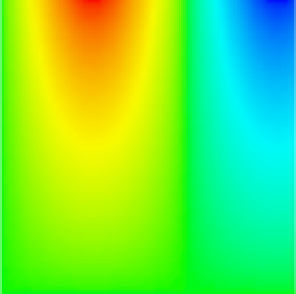
\includegraphics[scale=0.6]{figures/f_expxsinxt_60x60/f_expxsinxt_60x60_t0p5.pdf}
  \caption{The source function $f(x, y, t) = \exp(-t)y\sin(10xt)$, plotted with a $60 \times 60$ space coordinate mesh at the time $t = 0.5$.} \label{fig:f_t0.5}
\end{figure}

\begin{figure} 
  \centering
  
\includegraphics[scale=0.2]{figures/mesh/mesh3-crop.pdf}
  \caption{A two-dimensional finite element mesh, as used in our calculations.}\label{fig:mesh}
\end{figure}

In Fig. \ref{fig:t5}, we have plotted a snapshot of a solution $u_{h}$ taken at the time $t = 0.5$. When comparing the solutions with $20 \times 20$ and $60 \times 60$ mesh points, the results look very similar, at least to the eye. The wave length in $\sin(10xt)$ is inversely proportional with $t$, and the function $f$ therefore induces waves with longer wave lengths when $t$ is small. The solution is therefore smooth, and dominated by the initial Gaussian function. This domain seems to be easy to handle for the finite element method.

\begin{figure}
  \centering
  \mbox{
    \subfigure[]{
      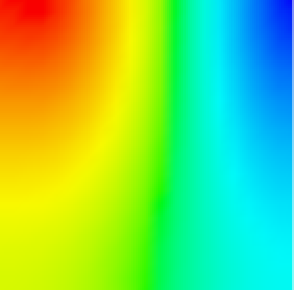
\includegraphics[width=.2\textwidth]{figures/expxsinxt_20x20/gaussian_expxsinxt_t5.pdf}
    }\quad
    \subfigure[]{
      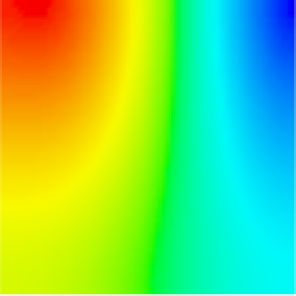
\includegraphics[width=.2\textwidth]{figures/expxsinxt_60x60/gaussian_expxsinxt_60x60_t5.pdf}
    }
  }
  \centering
  \caption{A snapshot of the solution $u_{h}$ taken at the time $t = 0.5$. Both calculations were done with P1 finite elements. Left: $20 \times 20$ mesh. Right: $60 \times 60$ mesh. Both solutions appear to be similar, at least when inspected by the eye.} \label{fig:t5}
\end{figure}

\begin{figure} 
  \centering
  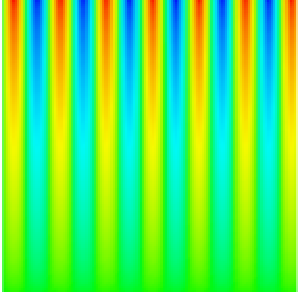
\includegraphics[scale=0.6]{figures/f_expxsinxt_100x100/f_expsinxt_100x100.pdf}
  \caption{The source function $f(x, y, t) = \exp(-t)y\sin(10xt)$, plotted with a $100 \times 100$ space coordinate mesh at the time $t = 4$.} \label{fig:f_t4}
\end{figure}


\begin{figure} 
  \centering
  \mbox{
    \subfigure[]{
      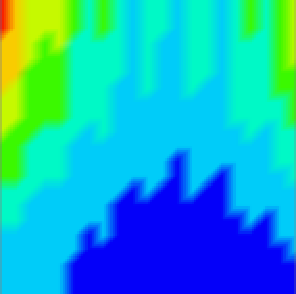
\includegraphics[width=.2\textwidth]{figures/expxsinxt_20x20/gaussian_expxsinxt2.pdf}
    }\quad
    \subfigure[]{
      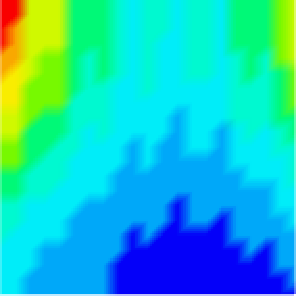
\includegraphics[width=.2\textwidth]{figures/expxsinxt_20x20_P2/gaussian_expxsinxt_20x20_P2.pdf}
    }
  }
  \centering
  \caption{Here the solution $u_{h}$ is plotted at the time $t = 4$. The number of space grid points was $20 \times 20$. The solution at left was obtained with P1 elements, whereas the solution at right was obtained with P2 finite elements.} \label{fig:t4_Nx20}
\end{figure}


\begin{figure}
  \centering
  \mbox{
    \subfigure[]{
      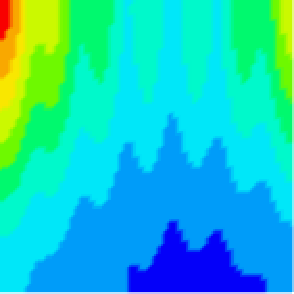
\includegraphics[width=.2\textwidth]{figures/expxsinxt_60x60/gaussian_expxsinxt_60x60.pdf}
     
    }\quad
    \subfigure[]{
      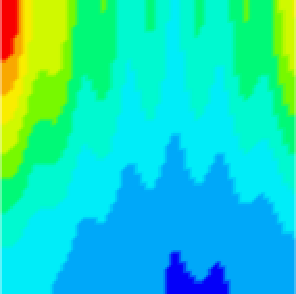
\includegraphics[width=.2\textwidth]{figures/expxsinxt_60x60_P2/gaussian_expxsinxt_60x60_P2.pdf}
    }
  }
  \centering
  \caption{The same calculations as visualized in Fig. \ref{fig:t4_Nx20}, but here with $60 \times 60$ space mesh points.} \label{fig:t4_Nx60}

\end{figure}

\begin{figure}
  \centering
  \mbox{
    \subfigure[]{
      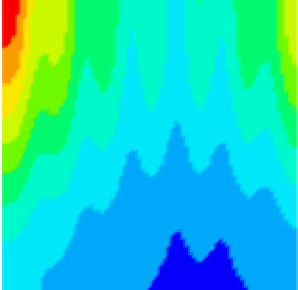
\includegraphics[width=.2\textwidth]{figures/expxsinxt_80x80/gaussian_expxsinxt_80x80.pdf}
     
    }\quad
    \subfigure[]{
      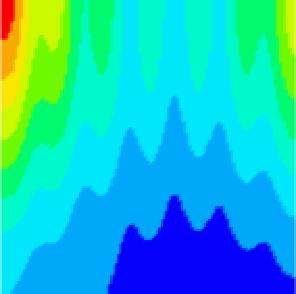
\includegraphics[width=.2\textwidth]{figures/expxsinxt_100x100/gaussian_expxsinxt_100x100.pdf}
    }\quad 
    \subfigure[]{
      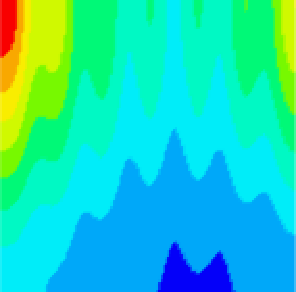
\includegraphics[width=.2\textwidth]{figures/expxsinxt_120x120/gaussian_expxsinxt_120x120.pdf}
    }
  }
  \centering
  \caption{The solution $u_{h}$ at time $t = 4$, as calculated with P1 elements. Left: $80 \times 80$ mesh points. Center: $100 \times 100$ mesh points. Right: $120 \times 120$ mesh points. As seen, the result is not converged with $100 \times 100$ mesh points.}

\end{figure}

At the time $t = 4$ the source function $f$ is much more complicated, as can be seen from Fig. \ref{fig:f_t4}. The rapid oscillations in $f$ gives rise to problems in the finite element solution. In Fig. \ref{fig:t4_Nx20} we have plotted the solution as obtained with $20 \times 20$ mesh points and P1 and P2 elements, at left and right, respectively. Both solutions are far from smooth, and they are quite different with P1 and P2 elements. The same case is repeated in Fig. \ref{fig:t4_Nx60}, but here with $60 \times 60$ space mesh points. Still with a $60 \times 60$ mesh, the P1 and P2 approximations give clearly different solutions. When increasing the number of grid points to $80 \times 80$, $100 \times 100$, and $120 \times 120$, and using P1 elements, the solution does not converge to the same visual picture. This is a bit surprising, since with 100 grid points there should be approximately 14 grid points per period of the function $f$, since $f$ has 7 wave crests in Fig. \ref{fig:f_t4}.    

As shown in Section 18 in the lecture notes, the diffusion equation discretized in time with the Backward Euler method gives a stable and non-oscillating solution provided the Courant number $C = \alpha \Delta t/\Delta x^{2}$ is a positive number. This is the case as long as $\alpha $ is positive. In the previous calculations, $\alpha $ was always positive. We did not either observe any instabilities in the results. For example with $\beta = 100$, which always gives a positive $\alpha$, we got a stable solution. When choosing $\beta = -100$, the solution became very instable.  

\section{Conclusions}

First, we set up numerical schemes for solving nonlinear diffusion equations, discretizing in time with a finite difference method and in space with finite elements. We showed how the Picard iteration and Newton's methods can be used to solve the nonlinear systems of equations. The combined finite difference and finite element method was implemented using Python and the FEniCS software package. The code was tested using the method of manufactured solutions. Finally, we studied a few example cases using the implementation. We got unstable solutions in some cases when the diffusion function $\alpha $ was allowed to become negative.  


\printindex

\begin{thebibliography}{1}
  \bibitem{fenics}
    A. Logg, K.-A. Mardal, G. N. Wells et al., \newline
    \newblock{\emph{Automated Solution of Differential Equations by the Finite Element Method}}, \newline
    \newblock{Springer, [doi:10.1007/978-3-642-23099-8].}

\bibitem{tutorial}
  H. P. Langtangen, \newline
  \newblock{\emph{A FEniCS Tutorial}}, \newline
  \newblock{\verb+http://fenicsproject.org/documentation/tutorial/index.html+}

\end{thebibliography}

\end{document}
